\ifx\allfiles\undefined
\documentclass[12pt, a4paper,oneside, UTF8]{ctexbook}
\usepackage[dvipsnames]{xcolor}
\usepackage{amsmath}   % 数学公式
\usepackage{amsthm}    % 定理环境
\usepackage{amssymb}   % 更多公式符号
\usepackage{graphicx}  % 插图
%\usepackage{mathrsfs}  % 数学字体
%\usepackage{newtxtext,newtxmath}
%\usepackage{arev}
\usepackage{kmath,kerkis}
\usepackage{newtxtext}
\usepackage{bbm}
\usepackage{enumitem}  % 列表
\usepackage{geometry}  % 页面调整
%\usepackage{unicode-math}
\usepackage[colorlinks,linkcolor=black]{hyperref}

\usepackage{wrapfig}


\usepackage{ulem}	   % 用于更多的下划线格式,
					   % \uline{}下划线,\uuline{}双下划线,\uwave{}下划波浪线,\sout{}中间删除线,\xout{}斜删除线
					   % \dashuline{}下划虚线,\dotuline{}文字底部加点


\graphicspath{ {flg/},{../flg/}, {config/}, {../config/} }  % 配置图形文件检索目录
\linespread{1.5} % 行高

% 页码设置
\geometry{top=25.4mm,bottom=25.4mm,left=20mm,right=20mm,headheight=2.17cm,headsep=4mm,footskip=12mm}

% 设置列表环境的上下间距
\setenumerate[1]{itemsep=5pt,partopsep=0pt,parsep=\parskip,topsep=5pt}
\setitemize[1]{itemsep=5pt,partopsep=0pt,parsep=\parskip,topsep=5pt}
\setdescription{itemsep=5pt,partopsep=0pt,parsep=\parskip,topsep=5pt}

% 定理环境
% ########## 定理环境 start ####################################
\theoremstyle{definition}
\newtheorem{defn}{\indent 定义}[section]

\newtheorem{lemma}{\indent 引理}[section]    % 引理 定理 推论 准则 共用一个编号计数
\newtheorem{thm}[lemma]{\indent 定理}
\newtheorem{corollary}[lemma]{\indent 推论}
\newtheorem{criterion}[lemma]{\indent 准则}

\newtheorem{proposition}{\indent 命题}[section]
\newtheorem{example}{\indent \color{SeaGreen}{例}}[section] % 绿色文字的 例 ,不需要就去除\color{SeaGreen}{}
\newtheorem*{rmk}{\indent \color{red}{注}}

% 两种方式定义中文的 证明 和 解 的环境:
% 缺点:\qedhere 命令将会失效【技术有限,暂时无法解决】
\renewenvironment{proof}{\par\textbf{证明.}\;}{\qed\par}
\newenvironment{solution}{\par{\textbf{解.}}\;}{\qed\par}

% 缺点:\bf 是过时命令,可以用 textb f等替代,但编译会有关于字体的警告,不过不影响使用【技术有限,暂时无法解决】
%\renewcommand{\proofname}{\indent\bf 证明}
%\newenvironment{solution}{\begin{proof}[\indent\bf 解]}{\end{proof}}
% ######### 定理环境 end  #####################################

% ↓↓↓↓↓↓↓↓↓↓↓↓↓↓↓↓↓ 以下是自定义的命令  ↓↓↓↓↓↓↓↓↓↓↓↓↓↓↓↓

% 用于调整表格的高度  使用 \hline\xrowht{25pt}
\newcommand{\xrowht}[2][0]{\addstackgap[.5\dimexpr#2\relax]{\vphantom{#1}}}

% 表格环境内长内容换行
\newcommand{\tabincell}[2]{\begin{tabular}{@{}#1@{}}#2\end{tabular}}

% 使用\linespread{1.5} 之后 cases 环境的行高也会改变,重新定义一个 ca 环境可以自动控制 cases 环境行高
\newenvironment{ca}[1][1]{\linespread{#1} \selectfont \begin{cases}}{\end{cases}}
% 和上面一样
\newenvironment{vx}[1][1]{\linespread{#1} \selectfont \begin{vmatrix}}{\end{vmatrix}}

\def\d{\textup{d}} % 直立体 d 用于微分符号 dx
\def\R{\mathbb{R}} % 实数域
\def\N{\mathbb{N}} % 自然数域
\def\C{\mathbb{C}} % 复数域
\def\Z{\mathbb{Z}} % 整数环
\def\Q{\mathbb{Q}} % 有理数域
\newcommand{\bs}[1]{\boldsymbol{#1}}    % 加粗,常用于向量
\newcommand{\ora}[1]{\overrightarrow{#1}} % 向量

% 数学 平行 符号
\newcommand{\pll}{\kern 0.56em/\kern -0.8em /\kern 0.56em}

% 用于空行\myspace{1} 表示空一行 填 2 表示空两行  
\newcommand{\myspace}[1]{\par\vspace{#1\baselineskip}}

%s.t. 用\st就能打出s.t.
\DeclareMathOperator{\st}{s.t.}

%罗马数字 \rmnum{}是小写罗马数字, \Rmnum{}是大写罗马数字
\makeatletter
\newcommand{\rmnum}[1]{\romannumeral #1}
\newcommand{\Rmnum}[1]{\expandafter@slowromancap\romannumeral #1@}
\makeatother
\begin{document}
	% \title{{\Huge{\textbf{$Real \,\, Analysis$}}}\\
		\Large{\textbf{$Measure \,\, Theory , \,\, Integration , \,\, \& \,\, Hilbert \,\, Spaces$}}\footnote{参考书籍:\\
			\hspace*{4em} \textbf{《$Real \,\, Analysis -- Measure \,\, Theroy, \,\, Integration, \,\, \& \,\, Hilbert \,\, Spaces$》--- $Elias \,\, M. \,\, Stein$} \\
			\hspace*{4em} \textbf{《$Real \,\, Analysis -- Modern \,\, Techniques \,\, and \,\, Their \,\, Applications$》--- $Gerald \,\, B. \,\, Folland$}}}
\author{$-TW-$}
\date{\today}
\maketitle                   % 在单独的标题页上生成一个标题

\thispagestyle{empty}        % 前言页面不使用页码
\begin{center}
	\Huge\textbf{序}
\end{center}


\vspace*{3em}
\begin{center}
	\large{\textbf{天道几何,万品流形先自守;}}\\
	
	\large{\textbf{变分无限,孤心测度有同伦。}}
\end{center}

\vspace*{3em}
\begin{flushright}
	\begin{tabular}{c}
		\today \\ \small{\textbf{长夜伴浪破晓梦,梦晓破浪伴夜长}}
	\end{tabular}
\end{flushright}


\newpage                      % 新的一页
\pagestyle{plain}             % 设置页眉和页脚的排版方式(plain:页眉是空的,页脚只包含一个居中的页码)
\setcounter{page}{1}          % 重新定义页码从第一页开始
\pagenumbering{Roman}         % 使用大写的罗马数字作为页码
\tableofcontents              % 生成目录

\newpage                      % 以下是正文
\pagestyle{plain}
\setcounter{page}{1}          % 使用阿拉伯数字作为页码
\pagenumbering{arabic}
\setcounter{chapter}{0}    % 设置 -1 可作为第零章绪论从第零章开始 
	\else
	\fi
	%  ############################ 正文部分
\chapter{$Measurable \,\, Functions$}
\section{$Measurable \,\, Functions$}
\paragraph{定义}
	下面给出$\R^d$ 上\textbf{可测函数}的定义.(注意值域为\uwave{\textbf{扩充实数系$\overline{\R}$}})
	\begin{defn}\label{def 2.1.1}
		A function defined on a measurable subset $E \subset \R^d$ is \underline{\textcolor{blue}{\textbf{measurable}}} if for all $a \in \R$,
		\begin{align}
			f^{-1}([-\infty , a)) = \{ x \in E \mid f(x) < a \}
		\end{align}
		is measurable.
		
		\begin{rmk}
			\begin{itemize}
				\item $f^{-1}([-\infty , a))$ 常简记作$\{ f < a \}$.
				
				\item 下面给出几条等价定义.
				\begin{enumerate}
					\item[(1)]$\{ f < a \}$ is measurable. $\Leftrightarrow$ $\{ f \leq a \}$ is measurable.
					
					\item[(2)]$\Leftrightarrow$ $\{ f > a \}$ is measurable $\Leftrightarrow$ $\{ f \geq a \}$ is measurable.
					
					\item[(3)]If f is finite-valued, then
					\begin{align}
						f \,\, is \,\, measurable \,\, \Leftrightarrow \,\, \{ a < f < b \} \,\, is \,\, measurable, \,\, \forall a , b \in \R
					\end{align}
				\end{enumerate}
			
				\vspace{2em}
				\begin{proof}
					\begin{enumerate}
						\item[(1)]Since the collection of measurable sets is closed under countable intersections and unions,
						\begin{align}
							\{ f \leq a \} &= \bigcap_{n = 1}^{\infty}{\{ f < a + \frac{1}{n} \}} \\
							\{ f < a \} &= \bigcup_{n = 1}^{\infty}{\{ f \leq a - \frac{1}{n} \}}
						\end{align}
						Therefore, $\{ f < a \}$ is measurable. $\Leftrightarrow$ $\{ f \leq a \}$ is measurable.
						
						\item[(2)]Since the collection of measurable sets is closed under complements, easily proof by (1).
						
						\item[(3)]Since f is finite-valued,
						\begin{align}
							\{ f < a \} &= \bigcup_{n = 1}^{\infty}{\{ -n < f < a \}} \\
							\{ a < f < b \} &= \{ f > a \} \cap \{ f < b \}
						\end{align}
						Therefore, by (2), $f$ is measurable $\Leftrightarrow$ $\{ a < f < b \}$ is measurable.
					\end{enumerate}
				\end{proof}
			\end{itemize}
		\end{rmk}
	\end{defn}

\vspace{2em}
\paragraph{Property}
	下面给出可测函数的一些性质.
	\begin{enumerate}
		\item[\textcolor{red}{\textbf{Property 1.}}]Let $-\infty < f(x) < +\infty$ (finite-valued), then
		\begin{align}
			f \,\, is \,\, measurable \,\, &\Leftrightarrow \,\, f^{-1}(O) \,\, is \,\, measurable \,\, \forall open \,\, set \,\, O \\
			&\Leftrightarrow f^{-1}(F) \,\, is \,\, measurable \,\, \forall closed \,\, set \,\, F
		\end{align}
	
		\vspace{2em}
		\begin{proof}
			$\forall O \underset{open}{\subset} \R$, there exists $\{ (a_n , b_n) \}_{n = 1}^{\infty}$, $\st$
			\begin{align}
				O = \bigcup_{n = 1}^{\infty}{(a_n , b_n)}
			\end{align}
			Then
			\begin{align}
				f^{-1}(O) = f^{-1}(\bigcup_{n = 1}^{\infty}{(a_n , b_n)}) = \bigcup_{n = 1}^{\infty}{f^{-1}((a_n , b_n))}
			\end{align}
			Since $f$ is finite-valued and measurable, then $f^{-1}(a_n , b_n)$ is measurable.\\
			Therefore, $f^{-1}(O)$ is measurable.
		\end{proof}
		
		\vspace{2em}
		\item[\textcolor{red}{\textbf{Property 2.}}]$\{ continuous \,\, functions \} \subset \{ measurable \,\, functions \}$
		\begin{enumerate}
			\item{(a)}If $f$ is continuous on $\R^d$, then $f$ is measurable.
			
			\item[(b)]If $f$ is measurable, finite-valued and $\Phi$ is continuous on $\R$, then $\Phi \circ f$ is measurable.
		\end{enumerate}
	
		\vspace{2em}
		\begin{proof}
			\begin{enumerate}
				\item[(a)]Since $f$ is continuous, $\forall O \underset{open}{\subset} \R$, $f^{-1}(O) \underset{open}{\subset} \R^d$. By Property 1, $f$ is measurable.
				
				\item[(b)]$\forall O \underset{open}{\subset} \R$. Since $\Phi$ is continuous, then $\Phi^{-1}(O)$ is open.\\
				Since $f$ is finite-valued and measurable, then $(\Phi \circ f)^{-1}(O) = f^{-1}(\Phi^{-1}(O))$ is open.\\
				Therefore, by Property 1, $\Phi \circ f$ is measurable.
			\end{enumerate}
		\end{proof}
		
		\vspace{2em}
		\item[\textcolor{red}{\textbf{Property 3.}}]Suppose $\{ f_n \}_{n = 1}^{\infty}$ is a sequence of measurable functions. Then
		\begin{align}
			\sup_{n}{f_{n}(x)} , \,\, \inf_{n}{f_{n}(x)} , \,\, \limsup_{n \to \infty}{f_{n}(x)} , \,\, \liminf_{n \to \infty}{f_{n}(x)}
		\end{align}
		are measurable.
		
		\begin{rmk}
			类比数列的上下极限,此处
			\begin{align}
				\limsup_{n \to \infty}{f_{n}(x)} &\coloneqq \lim_{k \to \infty}{\sup_{n \geq k}{\{ f_{n}(x) \}}} = \inf_{k}{\sup_{n \geq k}{\{ f_{n}(x) \}}} \\
				\liminf_{n \to \infty}{f_{n}(x)} &\coloneqq \lim_{k \to \infty}{\inf_{n \geq k}{\{ f_{n}(x) \}}} = \sup_{k}{\inf_{n \geq k}{\{ f_{n}(x) \}}}
			\end{align}
		\end{rmk}
		
		\vspace{2em}
		\begin{proof}
			Since
			\begin{align}
				\{ x \mid \sup_{n}{f_{n}(x)} > a \} &= \bigcup_{n = 1}^{\infty}{\{ x \mid f_{n}(x) > a \}} \\
				\{ x \mid \inf_{n}{f_{n}(x)} < a \} &= \bigcup_{n = 1}^{\infty}{\{ x \mid f_{n}(x) < a \}}
			\end{align}
			Then $\underset{n}{\sup}{f_{n}(x)} , \,\, \underset{n}{\inf}{f_{n}(x)}$ is measurable.\\
			Since $\underset{n \geq k}{\sup}{f_{n}(x)} , \,\, \underset{n \geq k}{\inf}{f_{n}(x)}$ are measurable, by the previous conclusion, then
			\begin{align}
				\limsup_{n \to \infty}{f_{n}(x)} = \inf_{k}{\sup_{n \geq k}{\{ f_{n}(x) \}}} \\
				\liminf_{n \to \infty}{f_{n}(x)} = \sup_{k}{\inf_{n \geq k}{\{ f_{n}(x) \}}}
			\end{align}
			are measurable.
		\end{proof}
	
		\newpage
		\item[\textcolor{red}{\textbf{Property 4.}}]If $\{ f_n \}_{n = 1}^{\infty}$ is a collection of measurable functions and
		\begin{align}
			\lim_{n \to \infty}{f_{n}(x)} = f(x)
		\end{align}
		then $f$ is measurable.
		
		\begin{rmk}
			\begin{itemize}
				\item 与数列上下极限相同,
				\begin{align}
					\lim_{n \to \infty}{f_{n}(x)} = f(x) \,\, \Leftrightarrow \,\, \limsup_{n \to \infty}{f_{n}(x)} = \liminf_{n \to \infty}{f_{n}(x)} = f(x)
				\end{align}
			
				\item 此 Property 即说明\uwave{\textbf{可测函数列对极限运算封闭}}. 注意到连续函数列对极限运算并不具备封闭性.(下面给出经典范例)
				\begin{example}\label{ex 2.1.1}
					\begin{align}
						\lim_{n \to \infty}{x^n} = 
						\begin{cases}
							0 , \,\, &0 \leq x < 1 \\
							1 , &x = 1
						\end{cases}
					\end{align}
				\end{example}
			\end{itemize}
		\end{rmk}
	
		\vspace{2em}
		\begin{proof}
			Since $\{ f_n \}_{n = 1}^{\infty}$ are measurable, $f(x) = \underset{n \to \infty}{\limsup}{f_{n}(x)} = \underset{n \to \infty}{\limsup}{f_{n}(x)}$,\\
			then according to Property 3, $f$ is measurable.
		\end{proof}
	
		\vspace{2em}
		\item[\textcolor{red}{\textbf{Property 5.}}]If $f$ and $g$ are measurable, then
		\begin{enumerate}
			\item[(\rmnum{1})]$f^k$, $k \in \N$ are measurable.
			
			\item[(\rmnum{2})]$f + g$ and $fg$ are measurable if both $f$ and $g$ are finite-valued.
		\end{enumerate}
	
		\vspace{2em}
		\begin{proof}
			\begin{enumerate}
				\item[(\rmnum{1})]Since
				\begin{align}
					\{ f^k > a \} &= \{ f > a^{\frac{1}{k}} \} , \,\, \forall k \,\, is \,\, odd \\
					\{ f^k > a \} &= \{ f > a^{\frac{1}{k}} \} \cup \{ f < -a^{\frac{1}{k}} \} , \,\, \forall k \,\, is \,\, even \,\, and \,\, a > 0
				\end{align}
				Therefore, $f^k$, $k \in \N$ are measurable.
				
				\item[(\rmnum{2})]Since\footnote{即必$\exists r \in \Q$, $\st \{ f + g > a \} \supset \{ f > a - r \} \cap \{ g > r \}$. (另一侧包含关系$\subset$ 显然易证)\\
				(反证. $\forall r \in \Q$ 上式不成立,则对于$r = 0 \in \Q$, $\exists x_0$, $\st f(x_0) > a , \,\, g(x_0) > 0$, 且$f(x_0) + g(x_0) \leq a$, 矛盾.)}
				\begin{align}
					\{ f + g > a \} = \bigcup_{r \in \Q}{\{ f > a - r \} \cap \{ g > r \}}
				\end{align}
				
				\newpage
				then $f + g$ is measurable.\\
				By the previous results in (\rmnum{1}) and (\rmnum{2}), since
				\begin{align}
					fg = \frac{1}{4} [ (f + g)^2 - (f - g)^2 ]
				\end{align}
				Therefore, $fg$ is also measurable.
			\end{enumerate}
		\end{proof}
	\end{enumerate}
	
	\vspace{2em}
	下面给出数学分析中曾介绍过的\textbf{几乎处处}的定义.
	\begin{defn}\label{def 2.1.2}
		A property or statement is said to hold \underline{\textcolor{blue}{\textbf{almost everywhere (a.e.)}}} if it is true except on a set of measure zero.
		
		\begin{example}\label{ex 2.1.2}
			\begin{align}
				f(x) = 
				\begin{cases}
					0 , \,\, &0 \leq x < 1 \\
					1 , &x = 1
				\end{cases}
			\end{align}
			We say $f$ is continuous a.e. on $[0 , 1]$ since $D(f) = \{ 1 \}$ has measure zero.
		\end{example}
	\end{defn}

	\vspace{2em}
	下面说明几乎处处相等可保持函数可测性.
	\begin{proposition}
		If $f$ is measurble and $f = g$ a.e. , then $g$ is measurable.
		
		\vspace{2em}
		\begin{proof}
			Since $f$ is measurable and
			\begin{align}
				g = (g - f) + f
			\end{align}
			then we shall proof that $g - f$ is measurable.\\
			Let $A \coloneqq \{ x \mid g(x) - f(x) \neq 0 \}$, then $m(A) = 0$. We get
			\begin{align}
				\forall a \geq 0, (g - f)^{-1}((-\infty , a]) = (\R^d \backslash A) \cup N , \,\, where \,\, N \subset A
			\end{align}
			Since $m(A) = 0$, then $N$ is measurable and $m(N) = 0$. So $(g - f)^{-1}((-\infty , a])$ is measurable.\\
			Therefore, $g - f$ is measurable. Then $g$ is measurable.
		\end{proof}
	\end{proposition}

\newpage
\section{$Measurable \,\, functions \,\, are \,\, nearly \,\, simple$}
	本节来介绍一个非常重要的定理. 即可测函数可由简单函数逼近.

\paragraph{特征函数}
	下面先来介绍\textbf{特征函数}的定义.
	\begin{defn}\label{def 2.2.1}
		If $E \subset \R$, the \underline{\textcolor{blue}{\textbf{characteristic / indicator function $\chi_E / \mathbbm{1}_E$}}}  of E is defined by
		\begin{align}
			\chi_E (x) = 
			\begin{cases}
				1 , \,\, &if \,\, x \in E \\
				0 , &if \,\, x \notin E
			\end{cases}
		\end{align}
	\end{defn}

	\vspace{2em}
	下面给出可测集与其对应特征函数的关系.
	\begin{proposition}\label{prop 2.2.1}
		$\chi_E$ is measurable $\Leftrightarrow$ $E$ is measurable
		
		\vspace{2em}
		\begin{proof}
			Since
			\begin{align}
				\chi_{E}^{-1}((-\infty , a]) = 
				\begin{cases}
					\varnothing , \,\, &a < 0 \\
					E^c , &0 \leq a < 1 \\
					\R^d , &a \geq 1
				\end{cases}
			\end{align}
			Then $E$ is measurable $\Rightarrow$ $\chi_E$ is measurable. \\
			$\chi_E$ is measurable $\Rightarrow$ $\chi_{E}^{-1}((-\infty , a]) = E^c$ is measurable. $\Rightarrow$ $E$ is measurable.
		\end{proof}
	\end{proposition}

	\vspace{2em}
	下面给出特征函数的基本性质.
	\begin{proposition}\label{prop 2.2.2}
		[Property].
		\begin{enumerate}
			\item[(1)]If $A \cap B = \varnothing$, then 
			\begin{align}
				\chi_{A \cup B} = \max{\{ \chi_A , \chi_B \}} = \chi_A + \chi_B
			\end{align}
			
			\item[(2)]$\chi_{A \cap B} = \min{\{ \chi_A , \chi_B \}} = \chi_A \cdot \chi_B$.
		\end{enumerate}
	\end{proposition}

\newpage
\paragraph{$Simple \,\, functions$}
	对特征函数做线性组合,即可得到\textbf{简单函数}.
	\begin{defn}\label{def 2.2.2}
		A \underline{\textcolor{blue}{\textbf{simple function}}} on $\R^d$ is a finite linear combination
		\begin{align}
			f(x) = \sum_{j = 1}^{n}{a_j \chi_{E_j}(x)}
		\end{align}
		where each $E_j$ is measurable and $m(E_j) < \infty$.
		
		\begin{rmk}
			此处定义中并未要求$\{ E_j \}_{j = 1}^{n}$ disjoint. 而事实上这便引出了下面介绍的\textbf{标准形式}.
		\end{rmk}
	\end{defn}

	\vspace{2em}
	下面的命题说明了每个简单函数都可写为\textbf{标准形式}($\{ E_j \}_{j = 1}^{n}$ disjoint).
	\begin{proposition}
		Every simple function $f$ has a \underline{\textcolor{blue}{\textbf{standard representaion}}}
		\begin{align}
			f = \sum_{k = 1}^{N}{a_k \chi_{E_k}} , \,\, where \,\, \{ E_j \}_{k = 1}^{N} \,\, are \,\, disjoint
		\end{align}
	
		\vspace{2em}
		\begin{proof}
			Suppose $f = \overset{N}{\underset{k = 1}{\sum}}{b_k \chi_{E_k}}$, $\{ E_j \}_{k = 1}^{N}$ may not be disjoint.\\
			Since $\{ E_j \}_{k = 1}^{N}$ is finite, the number of elements of range f is also finite. Suppose
			\begin{align}
				range \,\, f = \{ a_1 , \cdots , a_M \}
			\end{align}
			Then let $F_k = f^{-1}(\{ a_k \})$, then $\{ F_k \}_{k = 1}^{M}$ are disjoint. Therefore, we get the standard representation
			\begin{align}
				f = \sum_{k = 1}^{M}{a_k \chi_{F_k}}
			\end{align}
		\end{proof}
	\end{proposition}

\newpage
\paragraph{简单函数逼近可测函数}
	下面给出一个定理,说明任一可测函数可由简单函数列逼近.
	\begin{thm}\label{thm 2.2.1}
		Suppose $f : \R^d \longrightarrow [-\infty , \infty]$ is measurable. \\
		Then there exists a sequence $\{ \varphi_n \}$ of simple functions, $\st$
		\begin{align}
			&\varphi_1 \leq \varphi_2 \leq \cdots \leq f \\
			&\lim_{k \to \infty}{\varphi_{k}(x)} = f(x) , \,\, for \,\, all \,\, x
		\end{align}
		and $\varphi_k \to f$ uniformly on any set on which $f$ is bounded.
		
		\vspace{2em}
		\begin{proof}
			下面从两方面分类讨论,即非负函数$\&$ 变号函数,$f$ 有界$\&$ 无界.
			\begin{enumerate}
				\item[(1)]非负函数$f : \R^d \longrightarrow [0 , \infty]$.
				\begin{enumerate}
					\item[$1^{\circ}$]$f$ is bounded. Assume $\left| f(x) \right| \leq M$.\\
					Let\footnote{$E_{n}^k$ 表示第n次对值域进行分划后产生的第k个值域区间,其中$\frac{N_n + 1}{2^n} \geq M$.}
					\begin{align}
						E_{n}^{k} &= f^{-1}((\frac{k}{2^n} , \frac{k + 1}{2^n}]) , k = 0 , \cdots , N_n \\
						\varphi_{n}(x) &= \frac{k}{2^n} , \,\, if \,\, x \in E_{n}^{k}
					\end{align}
					Then
					\begin{align}
						\varphi_{n}(x) = \sum_{k = 0}^{N_n}{\frac{k}{2^n} \chi_{E_{n}^{k}}(x)}
					\end{align}
					Therefore\footnote{$\left| \varphi_{n}(x) - f(x) \right|$ 小于等于第n次分划后两个相邻值域区间的步长值,即$\frac{1}{2^n}$.}
					\begin{align}
						\left| \varphi_{n}(x) - f(x) \right| \leq \frac{1}{2^n} \to 0 \,\, (independent \,\, of \,\, x)
					\end{align}
					$\Rightarrow$ $\varphi_{n} \to f$ uniformly.
					
					\begin{figure}[htbp]  %h此处,t页顶,b页底,p独立一页,浮动体出现的位置
						\centering  %图表居中
						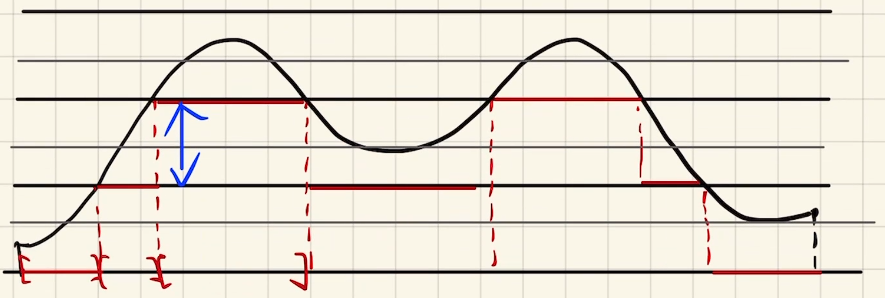
\includegraphics[width=0.55\textwidth]{figure/2.2-1} %图片的名称或者路径之中有空格会出问题 
						\caption{对$f$ 值域进行分划} % 图片标题
						\label{pic 2.1}
					\end{figure}
				
					\newpage
					\item[$2^{\circ}$]$f$ is unbounded. (\underline{idea}: truncation,将$f$ 截断为一列有界函数列,并逐点收敛于$f$)\\
					Let
					\begin{align}
						f_{k}(x) = 
						\begin{cases}
							f(x) , \,\, &if \,\, f(x) \leq k \\
							k , &if \,\, f(x) > k
						\end{cases}
					\end{align}	
					Then $f_{k}(x) \to f(x)$, $\forall x \in \R^d$. \\
					Since $f_k$ is bounded, by the previous result in $1^{\circ}$, \\
					For each $k$, $\exists$ a sequence of simple functions $\{ \psi_{kn} \}_{n = 1}^{\infty}$, $\st$
					\begin{align}
						\psi_{kn}(x) \to f_{k}(x) , \,\, \forall x
					\end{align}
					So we get
					\begin{align}
						\begin{matrix}
							&\textcolor{red}{\psi_{11}} \,\, &\psi_{12} \,\, &\psi_{13} \,\, &\cdots \,\, &\to \,\, &f_1 \\
							&\psi_{21} \,\, &\textcolor{red}{\psi_{22}} \,\, &\psi_{23} \,\, &\cdots \,\, &\to \,\, &f_2 \\
							&\psi_{31} \,\, &\psi_{32} \,\, &\textcolor{red}{\psi_{33}} \,\, &\cdots \,\, &\to \,\, &f_3 \\
							&\cdots \,\, &\cdots \,\, &\cdots \,\, &\cdots \,\, &\cdots \,\, &\cdots \\
							&\cdots \,\, &\cdots \,\, &\cdots \,\, &\cdots \,\, &\cdots \,\, &\downarrow \\
							& & & & & &\textcolor{red}{f} \\
						\end{matrix}
					\end{align}
					From the previous results in $1^{\circ}$, we get
					\begin{align}
						\left| \psi_{kn}(x) - f_k(x) \right| \leq \frac{1}{2^n}
					\end{align}
					Let $n = k$, then $\left| \psi_{kk}(x) - f_k(x) \right| \leq \frac{1}{2^k}$. Let $\varphi_k = \psi_{kk}$, then
					\begin{align}
						\left| \varphi_{k}(x) - f(x) \right| 
						\leq \left| \varphi_{k}(x) - f_{k}(x) \right| + \left| f_{k}(x) - f(x) \right|
					\end{align}
					Since $f_{k}(x) \to f(x)$, we get $\varphi_{k}(x) \to f(x)$, $\forall x$, where $\{ \varphi_k = \psi_{kk} \}_{k = 1}^{\infty}$ are simple functions.
				\end{enumerate}
				
				\item[(2)]变号函数$f : \R^d \longrightarrow [-\infty , \infty]$.\\
				We denote that
				\begin{align}
					f^{+}(x) &\coloneqq \max{\{ f(x) , 0 \}} \\
					f^{-}(x) &\coloneqq \max{\{ -f(x) , 0 \}}
				\end{align}
				By the previous results in (1), there exist sequences of simple functions $\{ \varphi_k \}_{k = 1}^{\infty} , \{ \psi_k \}_{k = 1}^{\infty}$, $\st$
				\begin{align}
					\varphi_k \to f^{+} \,\, and \,\, \psi_{k} \to f^{-} \,\, pointwisely
				\end{align}
				We can observe that $f = f^+ - f^-$ and $\left| f \right| = f^+ - f^-$.\\
				Let $\phi_{k}(x) = \varphi_{k}(x) - \psi_{k}(x)$, then $\phi_k$ is a simple function with $\phi_k \to f$ pointwisely.
			\end{enumerate}
		\end{proof}
	\end{thm}

\newpage
\paragraph{阶梯函数逼近可测函数}
	在证明了可测函数可由简单函数逼近后,我们更进一步,来说明可测函数可由更加简单的\textbf{阶梯函数}来逼近.
	
	\vspace{2em}
	先给出\textbf{阶梯函数}的定义.
	\begin{defn}\label{def 2.2.3}
		A \underline{\textcolor{blue}{\textbf{step function}}} is a finite sum
		\begin{align}
			f = \sum_{k = 1}^{N}{a_{k} \chi_{R_k}} , \,\, where \,\, R_k \,\, is \,\, a \,\, rectangle
		\end{align}
	
		\begin{rmk}
			阶梯函数$\&$ 简单函数的区别在于,简单函数是作用于有限个\textbf{可测集$E_k$},而阶梯函数是作用于有限个\textbf{矩形$R_k$}.
		\end{rmk}
	\end{defn}

	\vspace{2em}
	下面的定理说明了measurable functions are almost step functions.
	\begin{thm}\label{thm 2.2.2}
		Suppose $f$ is measurable on $\R^d$. Then there exists a sequence of step functions $\{ \psi_k \}_{k = 1}^{\infty}$, $\st$
		\begin{align}
			\lim_{k \to \infty}{\psi_{k}(x)} = f(x) , \,\, a.e. \,\, x
		\end{align}
	
		\begin{rmk}
			首先介绍函数列收敛点集的几种不同的等价表述:
			\begin{align}
				&\{ x \mid \forall \epsilon > 0 , \exists N \in \N , \forall n \geq N , \,\, \left| f_{n}(x) - f(x) \right| < \epsilon \} \\
				\Leftrightarrow 
				&\{ x \mid \forall n \in \N , \exists N \in \N , \forall k \geq N , \,\, \left| f_{k}(x) - f(x) \right| < \frac{1}{n} \} \\
				\Leftrightarrow 
				&\bigcap_{n = 1}^{\infty} \bigcup_{N = 1}^{\infty} \bigcap_{k = N}^{\infty} \{ x \mid \,\, \left| f_{k}(x) - f(x) \right| < \frac{1}{n} \}
			\end{align}
			从而可以得到函数列发散点集(Negation):
			\begin{align}
				&\{ x \mid \exists n \in \N , \forall N \in \N , \exists k \geq N , \,\, \left| f_{k}(x) - f(x) \right| \geq \frac{1}{n} \} \\
				\Leftrightarrow 
				&\bigcup_{n = 1}^{\infty} \bigcap_{N = 1}^{\infty} \bigcup_{k = N}^{\infty} \{ x \mid \,\, \left| f_{k}(x) - f(x) \right| \geq \frac{1}{n} \} \\
				\Leftrightarrow
				&\textcolor{red}{\bigcap_{N = 1}^{\infty} \bigcup_{k = N}^{\infty} \{ x \mid \,\, f_{k}(x) \neq f(x) \}}
			\end{align}
		\end{rmk}
	
		\vspace{2em}
		\begin{proof}
			(证明思路:先用阶梯函数逼近简单函数,再用简单函数逼近可测函数.)
			\begin{center}
				It suffices to show that $\chi_E$ can be approxiamted by step functions, for any measurable set $E$.
			\end{center}
			According to Thm\ref{thm 1.3.4} (\rmnum{4}) \\
			Let $f = \chi_E$, then $\forall \epsilon > 0$, $\exists$ cubes $\overset{N}{\underset{j = 1}{\bigcup}}{Q_j}$, $\st$
			\begin{align}
				m(E \,\, \triangle \,\, \bigcup_{j = 1}^{N}{Q_j}) \leq \epsilon
			\end{align}
			By considering the grid formed by extending the sides of these cubes, there exists almost disjoint rectangles $\{ \widetilde{R}_j \}_{j = 1}^{M}$, $\st$
			\begin{align}
				\bigcup_{j = 1}^{N}{Q_j} = \bigcup_{j = 1}^{M}{\widetilde{R}_j}
			\end{align}
			By taking ranctangles $R_j$ contained in $\widetilde{R}_j$, we can find a collection of disjoint rectangles $\{ R_j \}_{j = 1}^{M}$, $\st$
			\begin{align}
				m(E \,\, \triangle \,\, \bigsqcup_{j = 1}^{M}{R_j}) \leq 2\epsilon
			\end{align}
			For every $k \in \N$, there exists disjoint rectangles $\{ R_j \}_{j = 1}^{M}$, $\st$
			\begin{align}
				m(E \,\, \triangle \,\, \bigsqcup_{j = 1}^{M}{R_j}) \leq \frac{1}{2^{k + 1}}
			\end{align}
			There also exists a step function $\psi_k$
			\begin{align}
				\psi_{k}(x) \coloneqq \chi_{\bigcup_{j = 1}^{M}{R_j}}(x) = \sum_{j = 1}^{M}{\chi_{R_j}(x)}
			\end{align}
			Let
			\begin{align}
				E_k \coloneqq \{ x \mid f_{k}(x) \neq f(x) \}
			\end{align}
			Since $E_k \subset E \,\, \triangle \,\, \overset{M}{\underset{j = 1}{\bigsqcup}}{R_j}$, then $m(E_k) \leq \frac{1}{2^k}$. Let\footnote{根据\textcolor{red}{\textbf{注}}中式(2.56),$F$ 即为函数列$\{ \psi_k \}_{k = 1}^{\infty}$ 的发散点集,从而$\psi_{k}(x) \to f(x)$ 在$F^c$ 上收敛.}
			\begin{align}
				F_j = \bigcup_{j = k + 1}^{\infty}{E_j} , \,\, F = \bigcap_{k = 1}^{\infty}{F_k}
			\end{align}
			Then $\psi_{k}(x) \to f(x)$, $\forall x \in F^c$. Since
			\begin{align}
				m(F) &\leq m(F_k) , \,\, \forall k \in \N \\
				m(F_k) &= m(\bigcup_{j = k + 1}^{\infty}{E_j}) \leq \sum_{j = k + 1}^{\infty}{m(E_j)} \leq \frac{1}{2^k}
			\end{align}
			Therefore, $m(F) = 0$. $\underset{k \to \infty}{\lim}{\psi_{k}(x)} = f(x)$, $a.e.$ $x$.
		\end{proof}
	\end{thm}






	%  ############################
	\ifx\allfiles\undefined
\end{document}
\fi